\chapter{Stand der Forschung}
%TO DOs für dieses Kapitel: Abbildungen erstellen und einfügen und Zusammenfassung schreiben  

Dieses Kapitel legt die Grundlage für ein umfassendes Verständnis der Arbeit, indem relevante theoretische und technologische Konzepte sowie der aktuelle Forschungsstand dargestellt werden. Zunächst werden die Grundlagen von Virtual Reality erläutert, einschließlich der Definition von Virtual Reality und zentraler Begriffe wie Immersion und Presence. Zudem erfolgt eine Abgrenzung zu verwandten Begriffen und Konzepten wie Augmented Reality und Mixed Reality. Ergänzend werden grundlegende Informationen zu VR-Ausgabegeräten bereitgestellt, die eine technische Basis für das Verständnis der nachfolgenden Inhalte schaffen. Ein besonderer Schwerpunkt liegt auf dem Phänomen der Motion Sickness, da das Auftreten körperlicher Symptome eine häufige Herausforderung bei der Nutzung von VR-Anwendungen darstellt. 
Im weiteren Verlauf widmet sich das Kapitel dem aktuellen Forschungsstand zur Barrierefreiheit in VR. Zunächst werden bestehende Richtlinien vorgestellt. Anschließend werden Barrieren beleuchtet, die Menschen mit motorischen Beeinträchtigungen bei der Nutzung von VR-Anwendungen erfahren, und bestehende Lösungsansätze zur Überwindung dieser Barrieren präsentiert. Dabei wird auch auf Bereiche mit weiterem Forschungsbedarf hingewiesen.
Ein weiterer Abschnitt behandelt binäre Interaktionsschnittstellen als spezifische Lösung zur Verbesserung der Zugänglichkeit für Menschen mit motorischen Beeinträchtigungen. Hierbei werden zunächst verschiedene Arten von Schaltern beschrieben und anschließend gängige Scanning-Verfahren erläutert, die die Nutzung dieser Schalter ermöglichen.
Die Konzepte Usability und User Experience bilden eine wichtige Grundlage für die Bewertung von VR-Anwendungen. In diesem Zusammenhang werden etablierte Messmethoden wie der System Usability Scale (SUS) und der User Experience Questionnaire (UEQ) vorgestellt.
Anschließend wird das Tool PaneoVR eingeführt, das als Grundlage für die Implementierung der im Rahmen dieser Arbeit erarbeiteten Konzepte dient. Eine Zusammenfassung des Kapitels bietet einen abschließenden Überblick über den Stand der Forschung und leitet über zur Konzeption.

\section{Virtual Reality}

Der Begriff "Virtual Reality (VR)" wird in der Literatur nicht einheitlich definiert \citep{wohlgenannt_virtual_2020}. Es existieren verschiedene Definitionen, die unterschiedliche Aspekte der Technologie betonen. So wird VR beispielsweise von Berg und Vance als eine Sammlung von Technologien beschrieben, die es Menschen ermöglichen, immersiv eine Welt jenseits der Realität zu erleben. 
Nach \citet{bowman_virtual_2007} simuliert VR eine virtuelle Umgebung, die den Nutzenden das Gefühl vermittelt, "dort zu sein". \citet{jerald_vr_2016} definiert VR hingegen als eine computergenerierte digitale Umgebung, die erlebt und interagiert werden kann, als ob diese Umgebung real wäre. In ihrer Definition von VR führen \citet{wohlgenannt_virtual_2020} die verschiedenen Ansätze zur Beschreibung von VR zusammen und präzisieren, dass VR immersive Technologien nutzt, um interaktive virtuelle Umgebungen oder virtuelle Welten zu simulieren, in die sich die Nutzenden subjektiv einbringen und in denen sie sich physisch anwesend fühlen.

Des Weiteren identifizieren \citet{walsh_virtual_2002} Immersion, Interaktivität und Presence als drei zentrale Konzepte von VR. Der Begriff der Presence wird definiert als "die subjektive Erfahrung, sich an einem Ort oder in einer Umgebung zu befinden, auch wenn man physisch an einem anderen Ort ist" \citep{witmer_measuring_1998}. In einer virtuellen Umgebung entsteht das Gefühl von Presence insbesondere durch die Verlagerung der Aufmerksamkeit von der physischen auf die virtuelle Umgebung, wobei jedoch keine vollständige Ablösung von der physischen Realität notwendig ist \citep{witmer_measuring_1998}. 

Im Gegensatz zur Presence ist der Begriff der Immersion weniger eindeutig definiert. \citet{witmer_measuring_1998} beispielsweise definieren Immersion als einen psychologischen Zustand, in dem eine Person sich als umhüllt und in eine Umgebung eingebunden empfindet, die kontinuierliche Reize und Erfahrungen liefert. \citet{sanchez-vives_presence_2005} hingegen definieren Immersion als die technische Fähigkeit eines Systems, eine umfassende und überzeugende Umgebung zu erschaffen, mit der die Nutzenden interagieren können. 
Die Frage, ob Immersion als psychologischer Zustand oder als technische Eigenschaft des Systems zu verstehen ist, wirkt sich maßgeblich auf die Identifikation von Faktoren aus, die einen Einfluss auf die Immersion haben. 
Zu den wesentlichen Einflussfaktoren auf die Immersion zählen gemäß  \citet{sanchez-vives_presence_2005} unter anderem das Field of View, die Anzahl der simulierten sensorischen Systeme, die Qualität der Wiedergabe in jeder Sinnesmodalität, die Genauigkeit des Trackings, die Bildfrequenz und die Latenzzeit sowie die Übereinstimmung der simulierten sensorischen Daten mit der eigenen Körperwahrnehmung (Propriozeption). \citet{witmer_measuring_1998} hingegen definieren die Isolation von der physischen Umgebung, die Wahrnehmung der eigenen Einbindung in die virtuelle Umgebung, natürliche Interaktionsmodi sowie die Wahrnehmung der Eigenbewegung als relevante Einflussfaktoren. 

Neben diesen zentralen Konzepten betonen viele Definitionen die Bedeutung einer virtuellen Umgebung oder einer virtuellen Welt im Kontext von VR. Diese beiden Begriffe werden häufig in der Literatur verwendet, unterscheiden sich jedoch in ihrer Bedeutung. \citet{barfield_presence_1995} definieren eine virtuelle Umgebung als softwarebasierte Darstellungen realer (oder imaginierter) Agenten, Objekte und Prozesse sowie eine Mensch-Computer-Schnittstelle zur Darstellung und Interaktion mit diesen Modellen. Eine virtuelle Welt hingegen ist eine spezifische Form einer (multi-user) virtuellen Umgebung, die gemeinsame, simulierte Räume bietet, die von den Bewohnern, die als Avatare repräsentiert werden, bewohnt und gestaltet werden \citep{girvan_what_2018}.

Bei der Betrachtung des Themenbereichs Virtual Reality erfolgt eine häufige Bezugnahme auf verwandte Konzepte wie Mixed Reality oder Augmented Reality. Zur Klassifizierung und Abgrenzung aller Technologien, die Realität und Virtualität vereinen, entwarfen \citet{milgram_augmented_1995} das sogenannte Reality-Virtuality Continuum (RVC) (vgl. \autoref{fig:continuum}). 

\begin{figure}[tbh]
    \centering
    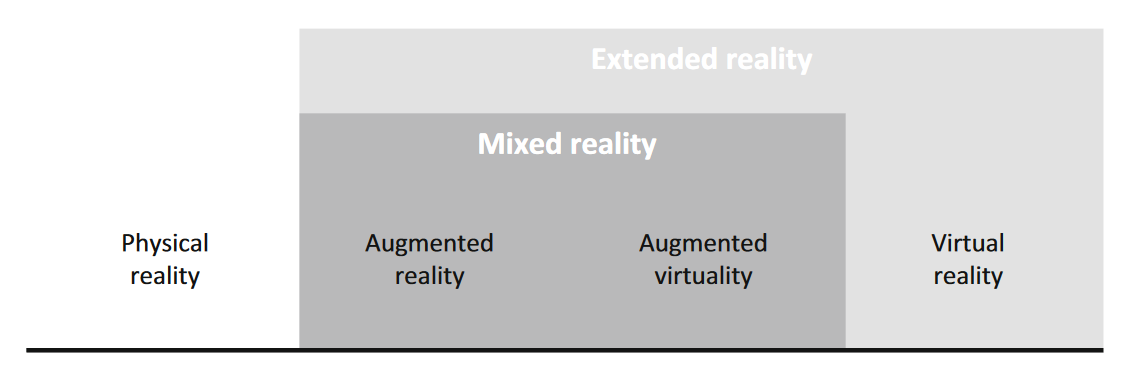
\includegraphics[width=0.95\textwidth]{images/Mixed-Reality-Cont-NEW.png}
    \caption{Reality-virtuality continuum nach \cite{wohlgenannt_virtual_2020}}
    \label{fig:continuum}
\end{figure}

Auf dem RVC bilden die reale Umgebung und die virtuelle
Umgebung die beiden Pole des Kontinuums. Die physikalische Realität setzt sich ausschließlich aus Elementen zusammen, welche durch eine Person direkt wahrgenommen werden können. Die virtuelle Umgebung, also die VR, besteht ausschließlich aus virtuellen Elementen. Der Nutzende wird dabei von der physikalischen Umgebung abgeschirmt, sodass er vollständig in die virtuelle Umgebung eintauchen kann. Der Bereich, der sich zwischen den beiden Polen des Kontinuums befindet, kombiniert virtuelle und physikalische Elemente und wird als Mixed Reality bezeichnet. Eine Umgebung, in der die physikalischen Elemente überwiegen, wird als Augmented Reality bezeichnet. Hierbei findet eine Erweiterung der physikalischen Realität durch virtuelle Elemente statt. Eine Erweiterung einer virtuellen Umgebung um physikalische Elemente wird demgegenüber als Augmented Virtuality bezeichnet. 
Ein weiterer Begriff, der in diesem Kontext häufig Verwendung findet, ist der Begriff der Extended Reality. Dieser wird häufig als Überbegriff verwendet und erfasst alle realen und virtuellen kombinierten Umgebungen und Mensch-Maschine-Interaktionen, die durch Computertechnologie und tragbare Geräte erzeugt werden \citep{fast-berglund_testing_2018}. \citet{wohlgenannt_virtual_2020} haben daher das ursprüngliche RVC um diesen Begriff erweitert (vgl. \autoref{fig:continuum}). 
 
Um virtuelle Umgebungen für die Nutzenden erfahrbar zu machen, werden sowohl Ausgabegeräte benötigt, die die virtuelle Umgebung darstellen, als auch Eingabegeräte, die die Interaktion mit dieser Umgebung ermöglichen. Ziel der Ausgabegeräte ist es, die virtuelle Welt so darzustellen, dass sie von den Nutzenden möglichst ähnlich wie die reale Welt wahrgenommen werden kann. Zu den am weitesten verbreiteten Ausgabegeräten zählen insbesondere sogenannte Head-Mounted Displays (HMDs). Dabei handelt es sich um Displays, die direkt am Kopf getragen werden und sich direkt vor den Augen der Nutzenden befinden. HMDs verfügen in der Regel über integrierte Trackingsysteme oder werden mit externen Trackinglösungen kombiniert, um die Position und Blickrichtung des Kopfes zu erfassen. Dies ermöglicht eine kontinuierliche Anpassung der virtuellen Kamera an die aktuelle Position und Orientierung des HMDs \citep{dorner_virtual_2019}. Darüber hinaus können aber bspw. auch Immersive Räume (CAVE) oder große Monitore Ausgabegeräte für VR-Anwendungen sein. Nach \citet{somrak_estimating_2019} können VR-Ausgabegeräte nach folgender Taxonomie beschrieben werden: 

\begin{itemize}
    \item Tragbare Geräte: 
    \begin{itemize}
        \item Mit einem Smartphone als Anzeige- und Verarbeitungseinheit (z.B. Google Cardboard)
        \item Eigenständige tragbare VR-Geräte (z.B. Meta Quest 3)
    \end{itemize}
    \item Kabelgebundene Geräte: 
    \begin{itemize}
        \item Geräte mit einer Kabelverbindung zu einem leistungsstarken Computer (z.B. HTC Vive)
    \end{itemize}
    \item Geräte, die an die Spielkonsole angeschlossen werden können (z.B. Sony PlayStation VR)
    \item Immersive Räume - CAVE (C-Automatic Virtual Environment)
    \item Große Monitore
\end{itemize}

Die Interaktion mit der virtuellen Umgebung erfolgt in der Regel über spezielle Eingabegeräte. Hier kommen insbesondere VR-Controller zum Einsatz. Alternativ oder ergänzend kann die Eingabe durch direktes Tracking von Körperteilen der Nutzenden, wie z.B. Finger, Hände, Arme oder Augen, erfolgen. In diesem Fall werden bspw. Gesten erkannt und in der virtuellen Umgebung als Eingaben interpretiert\citep{dorner_virtual_2019}.

\subsection{Motion Sickness}

Das Erleben von VR kann bei Nutzenden Symptome auslösen, die denen von Motion Sickness aus anderen Bereichen ähneln \citep{somrak_estimating_2019}. In der wissenschaftlichen Literatur werden neben dem Begriff "Motion Sickness" verschiedene Begriffe zur Beschreibung von unerwünschten Begleiterscheinungen virtueller Umgebungen verwendet. Dazu gehört der Begriff "Simulator Sickness", der insbesondere in den frühen militärischen Flugsimulatoren geprägt wurde \citep{kennedy_simulator_1993}, sowie "Cybersickness", das ursprünglich die Begleiterscheinungen virtueller Umgebungen allgemein beschrieb \citep{mccauley_cybersickness_1992}. In Studien mit HMDs findet zudem der Begriff "VR-Sickness" Verwendung (z.B. in \citep{kim_virtual_2018}). In der Forschung zu virtuellen Umgebungen werden diese Begriffe oft synonym verwendet, wobei eine spezifische Abgrenzung nicht erfolgt \citep{saredakis_factors_2020}. Im weiteren Verlauf dieser Arbeit wird der Begriff "Motion Sickness" verwendet. 

Das Spektrum der Symptome von Motion Sickness ist vielfältig. Zu den am häufigsten auftretenden Symptomen zählen unter anderem Unwohlsein, Apathie, Übelkeit, Schläfrigkeit, Desorientierung, Augenbelastung und Müdigkeit \citep{somrak_estimating_2019}. In besonders schweren Fällen können darüber hinaus Symptome wie Erbrechen, Schweißausbrüche, übermäßiger Speichelfluss, Schwindel, Magenschmerzen und völlige Arbeitsunfähigkeit auftreten \citep{kennedy_research_2010}. 

Die genauen Ursachen von Motion Sickness sind bislang nicht vollständig aufgeklärt. Eine der prominentesten Erklärungen liefert die Sensorische Konflikttheorie \citep{oman_motion_1990}. Diese besagt, dass die Symptome durch eine Diskrepanz zwischen visuellen, vestibulären und propriozeptiven Signalen entstehen. Diese Signale dienen in der Regel der Wahrnehmung der Ausrichtung und Bewegung des Körpers. In einer virtuellen Umgebung tritt jedoch häufig der Fall ein, dass der Körper visuell Bewegung wahrnimmt, während die vestibulären und propriozeptiven Systeme keine entsprechende Bewegung registrieren. Diese widersprüchlichen Signale führen zu sensorischen Diskrepanzen und können Motion Sickness auslösen. 

Als weitere Erklärungsansätze werden die Vergiftungstheorie sowie die Posturale Instabilitätstheorie diskutiert. Die Vergiftungstheorie besagt, dass der menschliche Körper bei der Aufnahme von Gift eine Reaktion auslöst, die das visuelle und vestibuläre System beeinflusst. In virtuellen Umgebungen können Reize das visuelle und vestibuläre System irritieren, sodass der Körper fälschlicherweise glaubt, Gift aufgenommen zu haben. Als Konsequenz treten unangenehme Symptome und eine Übelkeitsreaktion auf \citep{laviola_discussion_2000}. Die Posturale Instabilitätstheorie nach \citet{riccio_ecological_1991} basiert auf der Annahme, dass die Aufrechterhaltung der posturalen Stabilität in der Umgebung eines der Hauptziele menschlichen Verhaltens darstellt. Posturale Stabilität beschreibt den Zustand, in dem unkontrollierte Bewegungen der Wahrnehmungs- und Handlungssysteme minimiert werden. In virtuellen Umgebungen können abrupte oder signifikante Veränderungen zu einem Verlust der posturalen Kontrolle führen, insbesondere wenn die entsprechenden Kontrollstrategien noch nicht erlernt sind. Die Theorie besagt, dass anhaltende posturale Instabilität die Hauptursache für Motion Sickness ist. Je länger diese Instabilität andauert, desto schwerer sind die auftretenden Symptome.

Die Erfassung der Symptome von Motion Sickness erfolgt mittels subjektiver oder auch seltener objektiver Messmethoden \citep{somrak_estimating_2019}. Zu diesen objektiven Verfahren zählt die Messung physiologischer Veränderungen im menschlichen Körper, beispielsweise von Herzfrequenz, Blinkrate, Hauttemperatur oder Hirnstromaktivität (EEG), um Motion Sickness quantitativ zu erfassen \citep{somrak_estimating_2019}. Als Standard in der subjektiven Messung von Motion Sickness gilt der von \citet{kennedy_simulator_1993} entwickelte Simulator Sickness Questionnaire (SSQ) \citep{jerald_vr_2016}.

Der SSQ basiert auf der Einschätzung der Teilnehmenden, die nach der Nutzung einer Anwendung den Schweregrad von 16 verschiedenen Symptomen bewerten. Die Bewertung erfolgt auf einer Skala von 0 (keine Wahrnehmung) bis 3 (starke Wahrnehmung). Die erfassten Symptome lassen sich in die drei übergeordnete Kategorien Nausea (Übelkeit), Oculomotor disturbance (Okulomotorische Störungen) und Disorientation (Disorientierung) einteilen. Für jede dieser Kategorien wird ein separater Score berechnet, indem die Summen der Einzelbewertungen mit einem konstanten Gewichtungsfaktor multipliziert werden. 
Zusätzlich kann ein Gesamtscore berechnet werden, der alle drei Kategorien zusammenfasst. Höhere Gesamtscores und Scores in den einzelnen Kategorien deuten auf eine stärkere Wahrnehmung der entsprechenden Symptome hin und sind daher nicht erstrebenswert \citep{kennedy_simulator_1993}.

Zur Interpretation der Scores werden häufig die Grenzwerte nach \citet{stanney_cybersickness_1997} herangezogen. Diese beruhen auf Erkenntnissen, die aus einer umfangreichen Datenbasis von Militärpiloten gewonnen wurden. Die Grenzwerte der Gesamtscores liegen bei < 5 (vernachlässigbar), 5-10 (minimal), 10-15 (signifikant) und 15-20 (besorgniserregend). Anwendungen, die Gesamtscores von über 20 erzeugen, werden demnach als problematisch eingestuft. Es ist jedoch zu beachten, dass diese Schwellenwerte aus Daten von Militärpiloten abgeleitet wurden, die möglicherweise weniger anfällig für Motion Sickness sind als die Allgemeinbevölkerung. In vielen Evaluationen von VR-Anwendungen werden daher häufig durchschnittliche Scores von über 20 beobachtet \citep{bimberg_usage_2020}. Hohe Scores können u.a. darauf zurückzuführen sein, dass aufgrund der Gewichtungsfaktoren bereits geringe Zunahmen einzelner Symptome ausreichen, um diesen Schwellenwert zu überschreiten. Daher sollte die Interpretation von VR-Anwendungen anhand der Grenzwerte von \citet{stanney_cybersickness_1997} mit kritischem Blick erfolgen. 

Darüber hinaus ist eine Annahme des SSQ, dass die Teilnehmenden vor der Nutzung einer Anwendung völlig symptomfrei sind. In der Praxis ist dies jedoch schwer zu gewährleisten, da Symptome durch externe Faktoren wie Tageszeit, Anreise oder Stimmung beeinflusst werden können. Um den Einfluss der Anwendung auf das Auftreten von Motion Sickness genauer messen zu können, wird der SSQ häufig sowohl vor als auch nach der Nutzung durchgeführt, um anschließend die daraus resultierenden Unterschiede betrachten zu können \citep{bimberg_usage_2020}. \citet{kennedy_simulator_1993} kritisieren jedoch die geringe Zuverlässigkeit von Differenzwerten und schlagen vor, die Testpersonen stattdessen zu Beginn direkt zu fragen, ob sie sich in ihrem üblichen Gesundheitszustand befindet oder sich in irgendeiner Form krank fühlt. Personen, die sich nicht in ihrem üblichen Gesundheitszustand befinden sollten von der Analyse des SSQ folgend ausgeschlossen werden \citep{jerald_vr_2016}.

\section{Barrierefreiheit in VR} 

Die Forschung zur Barrierefreiheit in VR ist ein noch junges Forschungsgebiet, das besonders in den letzten Jahren zunehmend an Aufmerksamkeit gewonnen hat. Häufig konzentrieren sich die Studien auf eine bestimmte Form der Barriere oder Beeinträchtigung, wie Seh-, Hör-, motorische oder kognitive Beeinträchtigungen. Dabei werden die spezifischen Probleme und Herausforderungen identifiziert sowie entsprechende Konzepte und Lösungsansätze erarbeitet. Da sich diese Arbeit auf Menschen mit motorischen Beeinträchtigungnen bezieht, liegt der Fokus im Folgenden auf dem aktuellen Forschungsstand in diesem Bereich.

Für die meisten Softwareprodukte wie Webseiten, Apps oder Spiele existieren Richtlinien zur Barrierefreiheit, die Entwickler:innen bei der Gestaltung neuer Produkte und Systeme als Orientierung dienen können, um Barrierefreiheit zu gewährleisten. Wie \citet{heilemann_accessibility_2021} feststellen, berücksichtigen die meisten dieser Richtlinien jedoch kaum die spezifischen Anforderungen der Barrierefreiheit in virtuellen Umgebungen. Sie sind häufig auf bestimmte Beeinträchtigungen oder Geräte ausgerichtet und basieren auf Interaktionsmodellen, die nicht direkt auf VR-Anwendungen übertragbar sind. Die Interaktionsweise mit VR-Systemen unterscheidet sich grundlegend von anderen Softwarearten, sodass bestehende Leitlinien nur begrenzt auf VR übertragen werden können. Ein Fortschritt in diesem Bereich ist der Bericht der XR Association (XRA) aus dem Oktober 2020, der explizite Empfehlungen für die Entwicklung barrierefreier VR- und AR-Anwendungen enthält. Darin wird betont, dass Barrierefreiheit von Beginn an in den Designprozess integriert werden sollte. Meta hat in den sogenannten Virtual Reality Check (VRC)-Richtlinien \citep{meta_meta_2024} ebenfalls Abschnitte zur Barrierefreiheit aufgenommen. Diese Richtlinien, die jedoch nicht verpflichtend sind, um Produkte im Meta Quest Store anzubieten, umfassen derzeit nur neun Punkte. Zu den Empfehlungen zählen unter anderem die Möglichkeit der Steuerung mit nur einer Hand, Anpassungsoptionen für Anzeigeeinstellungen wie Helligkeit und Kontrast sowie die Bereitstellung verschiedener Fortbewegungsstile. Ein weiterer Ansatz ist die Gründung von XR Access \citep{xr_access_-_virtual_augmented__mixed_reality_for_people_with_disabilities_xr_2024}, einer Initiative aus Partnern von Universitäten und der Industrie. Ziel von XR Access ist es, inklusives Design und Barrierefreiheit zu grundlegenden und selbstverständlichen Bestandteilen der XR-Entwicklung zu machen. Darüber hinaus haben \citet{heilemann_accessibility_2021} in einer umfassenden Übersichtsarbeit bestehende Richtlinien zur Barrierefreiheit von VR-Spielen analysiert und zusammengefasst. In Bezug auf motorische Einschränkungen werden mehrere Empfehlungen hinsichtlich der Eingabe gegeben. Es wird betont, dass eine Möglichkeit zur Neuzuweisung oder Neukonfiguration der Steuerungen vorhanden sein sollte. Außerdem sollten Handbewegungen wie Kneifen, Drehen oder starkes Greifen vermieden werden. Stattdessen sollten einfache Steuerungsschemata angeboten werden. Des Weiteren wird empfohlen, die Kompatibilität mit assistiven Technologien wie Schaltern sicherzustellen und mehrere Eingabegeräte gleichzeitig zu unterstützen. Darüber hinaus sollte darauf geachtet werden, Auslöser für Motion Sickness zu vermeiden oder zumindest eine Option zur Deaktivierung solcher Auslöser bereitzustellen. Die Steuerung sollte nicht ausschließlich auf Bewegungserkennung, Kopfrotation oder bestimmte Körpertypen angewiesen sein.

\subsection{Barrieren für Menschen mit motorischen Beeinträchtigungen bei der Nutzung von VR}

Die Nutzung von VR-Anwendungen kann für Menschen mit motorischen Beeinträchtigungen eine Herausforderung darstellen. Bewegungsbasierte Interaktionen, die in VR häufig erforderlich sind, sind für viele Betroffene nur eingeschränkt oder gar nicht durchführbar. Diese Barrieren können nicht nur die Nutzbarkeit der Anwendungen einschränken, sondern den Zugang zu virtuellen Erlebnissen grundsätzlich erschweren. In der wissenschaftlichen Literatur wurden Probleme identifiziert, die im Zusammenhang mit motorischen Einschränkungen und der Interaktion mit virtuellen Umgebungen stehen. Im Folgenden wird der aktuelle Forschungsstand zu diesen Barrieren zusammengefasst,. 

Insgesamt können drei Kategorien von Barrieren identifiziert werden.

{\normalfont \bfseries 1. Einrichtung und Nutzung von VR-Ausgabegeräten}  

Ein grundlegendes Problem für Menschen mit motorischen Beeinträchtigungen bei der Nutzung von VR-Anwendungen stellt bereits die Einrichtung des Geräts dar, da dieser Prozess oft einen hohen körperlichen Einsatz oder auch feine motorische Fähigkeiten erfordert \citep{gerling_critical_2021}. So kann bereits das Einlegen der Batterien in die VR-Controller, das Anschließen von Kabeln an den Computer oder das Festlegen des räumlichen Brenzungsradius eine Barriere darstellen \citep{mott_i_2020}. Auch das eigenständige Auf- und Absetzen eines VR-HMD sowie das Einstellen des Kopfbandes kann für Personen mit eingeschränkter Beweglichkeit der Arme oder des Oberkörpers eine erhebliche Herausforderung darstellen \citep{mott_i_2020}. Eine zusätzliche Barriere stellen HMDs mit Kabelverbindung zum Computer dar. Dies gilt sowohl für die Einrichtung des Gerätes als auch für die Nutzung. So kann es z.B. vorkommen, dass Personen die einen Rollstuhl benutzen, versehentlich über die Kabel fahren oder sich diese in den Reifen verfangen \citep{mott_i_2020, wong_survey_2017}. 

{\normalfont \bfseries 2. Annahmen in Bezug auf den Körper} 
 
Die umfangreichen Anforderungen an die körperliche Beteiligung, die VR-Technologie stellt, können Barrieren für Menschen schaffen, die ihren Körper auf andere Weise in das System einbringen \citep{gerling_critical_2021}. Die geforderten Körperbewegungen basieren oft auf Fähigkeiten und Funktionen nicht-behinderter Personen. Dazu gehören bspw. die Nutzung im Stehen sowie die Verwendung von Gesten und beiden Händen zur Interaktion mit virtuellen Objekten \citep{wong_survey_2017}. VR-Anwendungen haben oft Probleme, Körper zu verfolgen und zu erfassen, die vom „Standard“ abweichen \citep{wong_survey_2017}. Darüber hinaus basieren auch anwendungsinterne Anforderungen an Energie und Ausdauer auf den Fähigkeiten von Menschen ohne Behinderungen \citep{wong_survey_2017}. Dies kann bei Menschen mit körperlichen Einschränkungen zu körperlicher, geistiger und zeitlicher Ermüdung führen. Als Folge können Schmerzen auftreten oder bereits bestehende körperliche Symptome sich verschlimmern \citep{creed_inclusive_2023}. Personen, die unter Erschöpfung oder chronischen Schmerzen leiden, könnten dadurch unter Umständen gänzlich von der Nutzung ausgeschlossen werden \citep{wong_survey_2017}. Ein weiteres Problem, das aus diesen Annahmen resultiert, ist, dass VR-Anwendungen in der Regel die Integration von assistiven Technologien nicht unterstützen bzw. mit diesen nicht kompatibel sind. Dies kann dazu führen, dass Nutzende weniger (Selbst-)Sicherheit bei der Anwendung empfinden \citep{creed_inclusive_2023}. 

{\normalfont \bfseries 3. Interaktion mit VR-Controllern} 

Die Nutzung gängiger VR-Controller stellt für Personen mit motorischen Beeinträchtigungen eine erhebliche Herausforderung dar. Aktuelle VR-Systeme sind in erster Linie für Personen konzipiert, die zwei Hände verwenden, lange stehen und virtuelle Objekte mit Hilfe der Hände manipulieren können. Diese Anforderungen schließen viele Menschen mit motorischen Beeinträchtigungen grundsätzlich von der Nutzung aus \citep{dombrowski_designing_2019}. Zusätzlich wird in VR-Anwendungen oftmals der gesamte Bewegungsradius der Nutzenden ausgenutzt und es werden Eingaben über Kopfhöhe sowie Bewegungen und Drehungen des Oberkörpers gefordert \citep{gerling_critical_2021}. Insbesondere die Nutzung von VR-Controller setzt dabei voraus, dass Nutzende eine oder beide Hände mit vollständiger Finger-, Handgelenks- und Armbeweglichkeit zur Verfügung haben \citep{mott_accessible_2019}. Daher haben viele Nutzende mit motorischen Beeinträchtigungen Schwierigkeiten, die Tasten auf den Controllern zu erreichen, zu drücken und gedrückt zu halten, insbesondere wenn gleichzeitig mehrere Tasten betätigt werden müssen \citep{mott_i_2020}. Insgesamt werden VR-Controller in der Regel nach dem Prinzip „One size fits all“ konzipiert sind, wodurch es an Flexibilität und Anpassungsfähigkeit für Nutzende mangelt \citep{creed_inclusive_2023}. Zusätzlich müssen die Controller stets im Sichtfeld der Headset-Kameras bleiben, damit ihre Position korrekt erfasst werden kann, was eine weitere Herausforderung darstellt \citep{mott_i_2020}. Für Personen, die nur wenig bis gar keine Beweglichkeit der Arme oder Hände haben, sind VR-Controller komplett unzugänglich \citep{mott_i_2020}. Darüber hinaus setzt der Einsatz von VR-Controllern voraus, dass die Nutzenden ihre Körperbewegungen jederzeit kontrollieren und daher bspw. präzise Selektionen vornehmen können. Dies ist jedoch nicht bei allen Menschen der Fall. Daher können unwillkürliche Körperbewegungen eine Herausforderung bei der Interaktion mit VR-Controllern darstellen. Diese Barriere gilt auch für Nutzende mit unwillkürlichen Augenbewegungen und ist besonders problematisch für VR-Anwendungen, bei denen konstante und zielgerichtete Augenbewegungen für die Interaktion erforderlich sind \citep{creed_inclusive_2023}. 

\subsection{Lösungsansätze zur Überwindung von Barrieren}

In der Literatur werden bereits einige Ansätze zur Verringerung der genannten Barrieren vorgestellt. So argumentieren \citet{mott_i_2020} bzgl. der Herausforderungen hinsichtlich gängiger HMDs, dass Drehknöpfe zum Anpassen des Kopfbandes näher an der Vorderseite des Headsets positioniert werden sollten, um die Erreichbarkeit zu verbessern. Eine automatische Anpassung des Kopfbandes anstelle einer manuellen Einstellung wird ebenfalls als hilfreich bewertet. Des Weiteren könnte die Verwendung eines kabellosen HMD eine einfache Lösung darstellen, um die Bewegungsfreiheit der Nutzenden zu erhöhen. Hinsichtlich der Interaktionsmöglichkeiten wird die Bereitstellung einer größeren Auswahl an Optionen und Anpassungsmöglichkeiten für Controller vorgeschlagen, um den unterschiedlichen Bedürfnissen der Nutzenden gerecht zu werden. Darüber hinaus könnten Eingabemethoden wie Sprachsteuerung und Blicksteuerung eine zugänglichere Alternative zu den herkömmlichen VR-Controllern darstellen. Des Weiteren wird vorgeschlagen, dass Nutzende die Möglichkeit haben sollten, Interaktionsmethoden oder Steuerungen neu zu konfigurieren, um eine individuellere Nutzung zu ermöglichen. \citet{dombrowski_designing_2019} führen aus, dass weitere potenzielle Verbesserungen die Steuerung von VR-Anwendungen mit alternativen Eingabegeräten wie Schaltern und die Verwendung von sich automatisch anpassenden Einstellknöpfen an VR-HMDs umfassen könnten. Darüber hinaus sollten Anwendungen und Eingabegeräte in der Lage sein, ungleichmäßige Eingaben zu tolerieren und versuchen, die Absicht des Nutzenden zu interpretieren. Das Design der Anwendung und die Interaktionsformen sollten effizient und komfortabel sein und mit minimaler Ermüdung genutzt werden können.

Neben diesen theoretischen Lösungsansätzen wurden in der Forschung bisher nur wenige praktische Untersuchungen hinsichtlich alternativer Interaktionsmethoden durchgeführt. Bei diesen Untersuchungen liegt der Fokus oftmals auf Sprach- und Blicksteuerung. Beispielsweise untersuchten und vergleichen \citet{minakata_pointing_2019} alternative Eingabeoptionen wie Kopf-, Blick- und Fußsteuerung hinsichtlich mentaler und physischer Anstrengung sowie Präzision. \citet{wang_intelligent_2018} entwickelten und evaluierten ein Eingabesystem, das auf Gesichtsausdrücken und Augenbewegungen basiert. \citet{10.1145/3441852.3471230} entwickelten Nearmi, ein Interaktionssystem, das darauf abzielt, die Bewegungen des Oberkörpers und des Kopfes zu reduzieren und das Auffinden und Erreichen von Points of Interest in der virtuellen Umgebung zu erleichtern. Dieses Framework basiert jedoch weiterhin überwiegend auf Eingaben mittels VR-Controller. \citet{valakou_framework_2024} entwickeln ein XR Accessibility Framework, das es Entwickler:innen erleichtern soll, verschiedene Barrierefreiheitsfunktionen in Anwendungen zu integrieren. Das Framework bietet unter anderem individuelle Texteinstellungen, interaktive Objektbeschreibungen und dynamisches Hervorheben von Kanten bei 3D-Objekten. Für Menschen mit motorischen Beeinträchtigungen, die Schwierigkeiten mit Point-and-Select Interaktionen haben, bietet das Framework zusätzlich eine Interaktionsmethode mittels sequentiellen Scanning. Dabei werden alle interaktiven Elemente in der Szene in einer hierarchischen Reihenfolge durchlaufen und hervorgehoben und können entsprechend ausgewählt werden.

Obwohl diese wenigen Ansätze bereits existieren, hat sich die Forschung bisher hauptsächlich auf die Identifizierung von Barrieren bei der Nutzung von VR-Anwendungen konzentriert. Insgesamt gibt es nur wenige Arbeiten zur Gestaltung und Entwicklung inklusiver VR-Anwendungen. Aus diesem Grund haben \citet{creed_inclusive_2024_2} eine Forschungsagenda für diesen Bereich erarbeitet, die die Kernbereiche hervorhebt, in denen weitere Forschung dringend erforderlich ist, um inklusivere AR- und VR-Anwendungen zu ermöglichen. In Bezug auf Menschen mit motorischen Beeinträchtigungen wurden z. B. die Erforschung alternativer Eingabemöglichkeiten (z. B. durch Blickverfolgung und Sprachsteuerung), die Untersuchung von Methoden zum Herausfiltern ungewollter und seltener auftretender Bewegungen (z. B. Stürzen, Taumeln, subtile repetitive Bewegungen wie Tremor) sowie die Untersuchung alternativer Ansätze für das Headset-Design, weitere Forschung zu anpassbaren Geräteschnittstellen und die Entwicklung von Hardwaresystemen, die gängige assistive Technologien integrieren und unterstützen können, identifiziert.

\section{Binäre Interaktionsschnittstellen}

Binäre Interaktionsschnittstellen bieten eine grundlegende Möglichkeit der Systemsteuerung durch einfache Eingaben. Dabei wird zwischen zwei Zuständen unterschieden, z.B. „An“ und „Aus“ oder „Gedrückt“ und „Nicht gedrückt“. Derartige Schnittstellen basieren auf der Verwendung von Schaltern (eng. Switches), die als assistive Technologien für Menschen mit motorischen Beeinträchtigungen entwickelt wurden, um die Verwendung von Mäusen, Tastaturen, Controllern oder Joysticks zu ersetzen, da diese oft schwer zugänglich sind. Schalter können prinzipiell mit jedem Körperteil bedient werden, das in der Lage ist, konsistente und willkürliche Bewegungen auszuführen. Die Art des verwendeten Schalters kann daher an die individuellen körperlichen Voraussetzungen einer Person angepasst werden. Während manche Menschen mit schweren motorischen Beeinträchtigungen nur einen Schalter bedienen können, sind andere in der Lage, mehrere Schalter parallel zu bedienen. Schalter können nach der Art der erforderlichen Aktion kategorisiert werden, wie z.B. Drücken, Ziehen, Kneifen oder durch Ein- und Ausatmen \citep{yuan_game_2011}, \citep{Weber22111996}. 

Im Folgenden werden verschiedene Arten von Schaltern sowie gängige Scanmethoden vorgestellt, die den Einsatz von Schaltern ermöglichen.

\subsection{Arten von Schaltern}

Schalter können auf verschiedene Weise aktiviert werden. \cite{COOK2015117} beschreiben drei grundlegende Möglichkeiten, wie Nutzende ein Signal an die Interaktionsschittstelle senden kann: Bewegung, Atmung und Phonation.

\textbf{Schalter basierend auf Bewegung}

Der häufigste Mechanismus zur Steuerung von Schaltern ist die Erkennung von Körperbewegungen. Dies kann durch verschiedene Arten von Schaltern erreicht werden.

\begin{itemize}
    \item \textit{Mechanische Schalter:}
    Mechanische Schalter reagieren auf Kraft, die durch Körperbewegungen erzeugt wird. Beispiele sind klassische Druckknöpfe oder Wippschalter. Einige Schalter erfordern eine sichtbare Bewegung (mechanische Verschiebung), während andere nur auf die ausgeübte Kraft reagieren. Mechanische Schalter sind vielseitig einsetzbar, aber aufgrund des erforderlichen Kraftaufwands möglicherweise nicht für Personen mit Muskelschwäche geeignet.
    \item \textit{Elektromagnetische Schalter:}
    Diese Schalter werden durch elektromagnetische Energie wie Licht oder Radiowellen aktiviert. Sie erfordern keinen direkten Körperkontakt und bieten somit eine berührungslose Steuerung. Ein Beispiel für elektromagnetische Schalter sind Lichtschranken.
    \item \textit{Elektrische Schalter:}
    Elektrische Schalter nutzen elektrische Signale, die vom menschlichen Körper erzeugt werden. Elektromyographische Signale (EMG), die bei Muskelkontraktionen entstehen, können mit Hilfe von Elektroden auf der Haut gemessen und zur Eingabe verwendet werden. Diese Schalter eignen sich besonders für Menschen mit Muskel- oder Bewegungsstörungen, da sie ohne mechanischen Aufwand bedient werden können. Auch Augenbewegungen und Hirnströme (z.B. in Brain-Computer-Interfaces, BCIs) können mit solchen Schaltern gemessen und zur Steuerung verwendet werden.
    \item \textit{Proximity-Schalter:}
    Proximity-Schalter registrieren Bewegungen ohne physischen Kontakt zum Körper. Dazu gehören z.B. Systeme zur Gestenerkennung oder wärmeempfindliche Schalter.   
\end{itemize}

\textbf{Schalter basierend auf Atmung}

Eine weitere Möglichkeit zur Erzeugung von Eingangssignalen ist die Nutzung der Atmung. Pneumatische Schalter, wie das weit verbreitete Sip-and-Puff-System, basieren auf der Erfassung von Luftdruck. Nutzende steuern das System durch Saugen („sip“) oder Blasen („puff“) in ein Röhrchen. Diese Technologie ist besonders nützlich für Menschen mit stark eingeschränkter Beweglichkeit.

\textbf{Schalter basierend auf Phonation}

Diese Kategorie umfasst Schalter, die auf Geräusche oder Sprache reagieren. Akustische Schalter können z. B. durch Klickgeräusche, regelmäßige Vokalisierungen oder konsistente Sprachlaute aktiviert werden. 
Diese Technologie eignet sich vor allem für Personen, die andere Eingabemethoden nicht nutzen können, aber über eine kontrollierte Lautproduktion verfügen.

\subsection{Scanning-Verfahren}
Scanning ist eine Eingabemethode, bei der dem Nutzenden eine Auswahl an Selektionsoptionen auf einem Display präsentiert wird. Sobald das gewünschte Element angezeigt wird, erfolgt eine Interaktion durch den Nutzenden, um dieses auszuwählen. Typischerweise wird dafür ein einzelner Schalter oder ein Array aus zwei oder mehr Schaltern verwendet. Scanning ermöglicht eine interaktive Steuerung, ohne dass umfangreiche motorische Fähigkeiten erforderlich sind \citep{COOK2015117}.

Es existieren diverse Scanning-Verfahren, die sich in der Art und Weise der Durchlaufung der Auswahlmöglichkeiten voneinander unterscheiden. Die gängigsten Verfahren sind dabei das Item Scanning, welches sich in den Unterarten Automatic, Step und Inverse Scanning differenziert, sowie das Continuous Cartesian Scanning.

Beim Item Scanning erfolgt eine sukzessive Hervorhebung einzelner Elemente. Die Selektion eines gewünschten Elements erfolgt durch Betätigung eines Schalters, sofern das entsprechende Zielelement hervorgehoben ist \citep{10.1145/772047.772049}. 

{\normalfont \bfseries Automatic Item Scanning} 

Beim Automatic Item Scanning erfolgt die Hervorhebung der Elemente automatisch. Die Hervorhebung bleibt bei jedem Element für ein vordefiniertes Zeitintervall stehen. Wird während der Hervorhebung eines Elementes eine Benutzereingabe vorgenommen, wird das hervorgehobene Element ausgewählt. Andernfalls wandert die Hervorhebung zum nächsten Element \citep{10.1145/772047.772049}.
Der wesentliche Vorteil des Automatic Item Scannings besteht in der Möglichkeit, die Interaktionen des Nutzenden auf ein Minimum zu reduzieren. Allerdings ist das Verfahren insgesamt relativ langsam. Des Weiteren erfordert es ein hohes Maß an sensorischer und kognitiver Aufmerksamkeit, um die Reihenfolge der Hervorhebung zu beobachten und zu verfolgen \citep{COOK2015117}.

{\normalfont \bfseries Step Item Scanning} 

Beim Step Item Scanning erfolgt die Hervorhebung der Elemente nicht automatisch, sondern durch wiederholte Aktivierung des Schalters durch den Nutzenden. Mit jeder Aktivierung erfolgt ein Sprung zur nächsten Auswahlmöglichkeit, bis das gewünschte Element erreicht ist. Die Selektion kann entweder mittels eines zusätzlichen Schalters getroffen werden, oder das System akzeptiert die Auswahl nach Ablauf einer festgelegten Zeitspanne (Dwell Selection). Ein wesentlicher Vorteil des Step Item Scannings besteht in der Möglichkeit, dass die Nutzenden die Geschwindigkeit der Hervorhebung selbst steuern können. Dadurch ist das Verfahren insgesamt schneller als das Automatic Item Scanning.  Allerdings ist zu berücksichtigen, dass dieses Vorgehen eine wiederholte Aktivierung des Schalters erfordert, was mit einer motorischen Ermüdung einhergehen kann \citep{COOK2015117}.

{\normalfont \bfseries Inverse Item Scanning} 

Die Initiierung des Inverse Scanning erfolgt durch Aktivierung und kontinuierliches Halten des Schalters. Solange die Betätigung des Schalters aufrechterhalten wird, erfolgt der Scan der Elemente. Sobald das gewünschte Element hervorgehoben wird, kann die Person den Schalter loslassen, um die Auswahl zu bestätigen. Inverse Scanning erfordert im Vergleich zum Step Scanning eine geringere Anzahl an Aktivierungen des Schalters, ist jedoch mit einer höheren sensorischen und kognitiven Aufmerksamkeit verbunden, da das Scanning kontinuierlich überwacht werden muss. Insbesondere für Personen, die einen erhöhten Zeitaufwand für die Initiierung und Ausführung von Bewegungen benötigen, kann dieses Verfahren von Vorteil sein \citep{COOK2015117}. 

{\normalfont \bfseries Continuous Cartesian Scanning}

Im Rahmen des Continuous Cartesian Scannings erfolgt das Scannen entlang orthogonaler Richtungen, bis das jeweilige Ziel erreicht ist. Eine horizontale Scanlinie beginnt mit einem kontinuierlichen Scan vom oberen Rand des Sichtfelds nach unten. Sobald die Scanlinie das Zielobjekt kreuzt, aktiviert der Nutzende den Schalter, wodurch die horizontale Linie an ihrer Position sichtbar bleibt. In der Folge wird eine vertikale Scanlinie initiiert, welche kontinuierlich von der linken Seite des Sichtfelds nach rechts scannt. Wenn auch die vertikale Scanlinie das Zielobjekt kreuzt, aktiviert der Nutzende den Schalter, um dieses Objekt auszuwählen \citep{Blackstien-Adler30062004}.

Der wesentliche Vorteil der Nutzung eines Scanning-Verfahrens liegt darin, dass eine Selektion von Elementen mit minimalem motorischen Aufwand realisierbar ist. Allerdings setzt die Nutzung dieser Methode gute visuelle Fähigkeiten, hohe Aufmerksamkeit sowie die Fähigkeit voraus, die Abfolge der Auswahlmöglichkeiten zu erfassen, insbesondere im Kontext des Item Scannings. Des Weiteren ist Scanning im Vergleich zu anderen Eingabemethoden relativ langsam. Um diesen Nachteil zu kompensieren, wurden verschiedene Ansätze zur Beschleunigung des Scannings entwickelt. Eine zentrale Methode ist das sogenannte Rate Enhancement beim Item Scanning, bei dem Elemente zu Gruppen zusammengefasst und selektiert werden können. Dadurch kann der Auswahlprozess signifikant beschleunigt werden \citep{COOK2015117}. 
Darüber hinaus stellt die Festlegung der optimalen Scangeschwindigkeit (Scan Rate) eine der größten Herausforderungen beim Scanning dar \citep{COOK2015117}. Beim Automatic und Inverse Item Scanning beschreibt die Scan Rate die Zeitspanne, während der ein Element für die Auswahl durch den Nutzenden hervorgehoben ist \citep{Simpson30062007}. Beim Continuous Cartesian Scanning ist die Scan Rate definiert als die Strecke, die der Scan in einer bestimmten Zeit zurücklegt \citep{Blackstien-Adler30062004}.Eine zu hohe Scan Rate kann dazu führen, dass Nutzende Schwierigkeiten haben, im richtigen Moment eine Auswahl zu treffen und dadurch viele Fehler machen oder das System gar nicht nutzen können. Eine zu niedrige Scan Rate hingegen verzögert den Eingabeprozess unnötig \citep{Simpson30062007}.  

\section{Usability und User Experience}

\textbf{Usability}
Der Begriff Usability, auch im Deutschen auch als Gebrauchstauglichkeit übersetzt, wird in der DIN-Norm EN ISO 9241-11:2018 wie folgt definiert:

\textit{„Ausmaß, in dem ein System, ein Produkt oder eine Dienstleistung durch bestimmte Benutzer in einem bestimmten Nutzungskontext genutzt werden kann, um bestimmte Ziele effektiv, effizient und zufriedenstellend zu erreichen.“ \cite{noauthor_din_nodate-1}.}

In den Anmerkungen zu dieser Definition wird verdeutlicht, dass die Gebrauchstauglichkeit immer in Bezug auf die Kombination aus spezifischen Benutzern, spezifischen Zielen und dem spezifischen Nutzungskontext betrachtet werden muss. Dies bedeutet, dass die Gebrauchstauglichkeit eines Systems, eines Produkts oder einer Dienstleistung in Abhängigkeit von den Zielen, der Art der Nutzenden und weiteren Aspekten des Nutzungskontextes unterschiedlich sein kann. Darüber hinaus wird präzisiert, dass sich der Begriff „Gebrauchstauglichkeit“ nicht nur auf die Qualität eines Systems bezieht, sondern auch als Qualifizierungsmerkmal verwendet wird, um Kompetenzen, Aktivitäten oder Methoden zur Verbesserung der Gebrauchstauglichkeit zu beschreiben. 

Im weiteren Verlauf dieser Arbeit wird der Begriff Usability verwendet, da dieser Begriff auch im Deutschen überwiegend verwendet wird. 

Die Messung der Usability basiert direkt auf den drei in der Definition verankerten Faktoren Effektivität, Effizienz und Zufriedenheit. Diese Merkmale können durch eine Vielzahl von Methoden erfasst werden, darunter Usability-Tests und speziell entwickelte Fragebögen. Ein bekanntes und weit verbreitetes Instrument zur Messung der Usability ist die System Usability Scale (SUS), die 1986 von John Brooke entwickelt und zehn Jahre später veröffentlicht wurde \citep{brooke_sus_1996}.

Die SUS besteht aus lediglich zehn Items und ist daher schnell und einfach durchzuführen. Anstelle einer differenzierten Bewertung einzelner Usability-Faktoren liefert die SUS einen Gesamtwert im Bereich von 0 bis 100. Zur Interpretation des SUS Scores werden üblicherweise die Ergebnisse von \citet{bangor_empirical_2008} herangezogen (vlg. \autoref{fig:susInterpretation}). Demnach liegt der durchschnittliche SUS Score bei 68. Scores unter 50 gelten als inakzeptabel, während Produkte mit einem Score von 70 oder höher als akzeptabel eingestuft werden. Bessere Produkte erreichen Werte zwischen 70 und 80, während herausragende Systeme Scores von über 90 erreichen. Produkte mit einem Score unter 70 sollten genauer überprüft und verbessert werden. 

\begin{figure}[tbh]
    \centering
    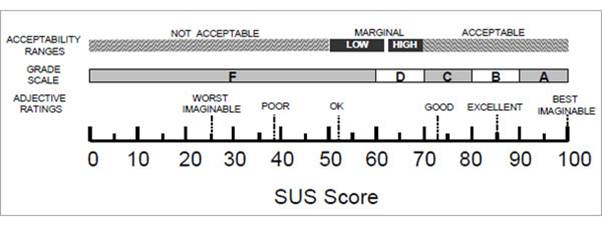
\includegraphics[width=0.95\textwidth]{images/SUS-Interpretation.jpg}
    \caption{Einstufung der SUS-Scores nach \citet{bangor_empirical_2008}}
    \label{fig:susInterpretation}
\end{figure}

\textbf{User Experience}

Neben der Usability ist auch die User Experience (UX) ein relevantes Konzept im Human Computer Interaction (HCI). Die DIN EN ISO 9241-210 definiert UX als \textit{„Wahrnehmungen und Reaktionen einer Person, die aus der tatsächlichen und/oder der erwarteten Benutzung eines Systems, eines Produkts oder einer Dienstleistung resultieren.“} \citep{noauthor_din_2020}. Die UX ist demnach essentiell, um nachvollziehen zu können, wie ein interaktives Produkt oder System von Nutzenden wahrgenommen wird. Damit hat sie gleichzeitig einen erheblichen Einfluss auf den Erfolg eines Produktes oder Systems. Fallen die Reaktionen und Wahrnehmungen der Nutzenden negativ aus, wird sich dies auf den Erfolg des Produkts auswirken. Die Definition der DIN-Norm bietet, im Gegensatz zur Usability, jedoch keine Kriterien zur Messung. Um die UX messbar zu machen, wird das Modell der pragmatischen und hedonischen Qualität nach \citet{hassenzahl_user_2008} verwendet. Danach setzt sich die UX aus der pragmatischen und der hedonischen Qualität zusammen. Unter pragmatischer Qualität wird die aufgabenbezogene Qualität eines Produktes verstanden. Ein Produkt besitzt pragmatische Qualität, wenn es Nutzende dabei unterstützt, Aufgaben effizient und effektiv zu erledigen. Die hedonische Qualität hingegen bezieht sich auf nicht aufgabenbezogene Aspekte eines Produktes. Dazu zählen beispielsweise Aspekte wie Einzigartigkeit und Originalität. Viele etablierte Methoden zur Evaluation der UX basieren auf dieser Unterscheidung von Qualitäten. 

Die meisten Messmethoden der UX wurden für 2D-Anwendungen, wie Websiten, Apps o.Ä. erstellt und validiert worden. Für VR-Anwendungen gibt es derzeit noch keine etablierten oder standardsierten Methoden zur Messung der UX \citep{alexandrovsky_evaluating_2021}. Am häufigsten werden jedoch quantitative Methoden zur Messung bei VR-Anwendungen eingesetzt \citep{kim_systematic_2020}. Ein häufig eingesetzter Fragebogen ist der User Experience Questionnaire \citep{laugwitz_construction_2008}. Dieser besteht aus 26 bipolaren Items und verwendet eine 7er Likert-Skala. Gemessen werden die UX-Faktoren Attraktivität, Druchschaubarkeit, Effizienz, Steuerbarkeit, Stimulation und Originalität. Der UEQ steht in über 20 Sprachen zur Verfügung. Der Fragebogen sowie ein spezifisches Auswertungstool kann kostenlos genutzt werden. 

\section{PaneoVR}

Das PaneoVR-Tool wurde entwickelt, um immersive 360°-Videotrainings bereitzustellen und die Erstellung virtueller Lehrinhalte für Bildungszwecke zu vereinfachen. Es handelt sich dabei um eine Web- und VR-Anwendung, die es Nutzenden ermöglicht, ohne tiefgehende Fachkenntnisse in Informatik oder Medientechnik ansprechende VR-Szenarien zu erstellen und zu nutzen \citep{noauthor_paneovr_nodate}. Das Konzept wurde im Rahmen des vom Bundesministerium für Bildung und Forschung geförderten Projekts ViRDiPA \citep{noauthor_virdipa-_nodate} entwickelt. Dieses Projekt lief vom 01.03.2020 bis 31.08.2023 und das Ziel bestand darin, VR als innovative Lehrmethode in der Pflegeausbildung zu etablieren. Die Entwicklung erfolgt in Zusammenarbeit mit dem Mixed Reality Lab der Hochschule Emden/Leer.

PaneoVR richtet sich an Personen, Unternehmen oder Einrichtungen, die eigenständig virtuelle Trainings ohne den Aufwand und die Kosten aufwendiger 3D-Designs und Animationen erstellen möchten. Stattdessen nutzt das Tool 360°-Videotechnik, die eine realitätsgetreue Darstellung auf einfache Weise ermöglicht. Diese Methode erlaubt es, Szenarien von einfachen Raumtouren bis hin zu komplexen Rollenspiel-Erlebnissen zu erstellen. Nutzende stehen innerhalb von Video- oder Fotosphären und können durch Interaktion mit digitalen Elementen Einfluss auf die Umgebung nehmen, was eine dynamische und immersive Erfahrung schafft.

Das Tool besteht aus drei wesentlichen Komponenten:

\begin{itemize}
    \item \textbf{Diagrammeditor/Webeditor:}
    Der nodebasierte Diagrammeditor bildet die zentrale Plattform zur Erstellung der VR-Szenarien. Nutzende können 360°-Videos, Bilder und Audiodateien hochladen und daraus interaktive Szenen gestalten und zu Szenarien verknüfpen. 
    \item \textbf{VR-Anwendung/PaneoVR App:}
    Die PaneoVR App läuft auf allen gängigen VR-Brillen und ermöglicht es, die erstellten Szenarien direkt in Virtual Reality zu durchlaufen. Zusätzlich bietet die App einen Editor-Modus, über den unter anderem die Positionierung interaktiver Elemente in der Szene angepasst werden kann. 
    \item \textbf{Web Player:}
    Als Alternative zur VR-Anwendung erlaubt der Web Player, die Szenarien auf einem Rechner zu durchlaufen oder zu bearbeiten.
\end{itemize}

PaneoVR bietet eine Vielzahl interaktiver Elemente, die es Nutzenden ermöglichen, Szenarien individuell und ansprechend zu gestalten. Die Basisfelder repräsentieren dabei die einfachsten Interaktionsmöglichkeiten und dienen der einfachen Navigation zwischen Szenen innerhalb eines Szenarios. Zu den Basisfeldernzählen die Elemente Wegpunkt, Benutzen und Textpunkt. Diese erlauben es, durch einen Klick zur jeweils verknüpften Szene zu wechseln. Die Elemente unterscheiden sich dabei nur in der Darstellung des Buttons und nicht in ihrer Funktionsweise. Auch automatische Wechsel können integriert werden. Hierbei erfolgt der Szenenwechsel automatisch nach Abschluss des laufenden Szenenvideos. Dieses Element wird in der Szene nicht dargestellt. 
Für komplexere und nicht-lineare Szenenwechsel stehen Verzweigungselemente zur Verfügung. Das Dialog-Element bietet bis zu vier verschiedene Multiple-Choice-Optionen, die beispielsweise als Antworten auf zuvor im Video gesagte Inhalte verwendet werden können. Jede Option kann mit einer nachfolgenden Szenen verknüpft und textlich dargestellt werden. Das Quiz-Element ähnelt dem Dialog, beinhalet jedoch eine zentrale Frage, die in der Mitte der  Multiple-Choice-Antworten dargestellt wird. Das Zufällig-Element wird in der Szene wie ein einfacher Wegpunkt dargestellt. Bei Auswahl dieses Elements wird jedoch zufällig eine der verknüpften Szenen ausgewählt, was eine dynamische Variation innerhalb eines Szenarios erlaubt.
PaneoVR bietet außerdem die Möglichekit, Bilder in die Szenen einzubinden und diese interaktiv zu nutzen. Ein Bild-Element bindet das gewählte Bild als Miniaturansicht in die Szene ein. Wird dieses ausgewählt, erscheint eine vergrößerte Ansicht des Bildes, die über einen Zurück-Button wieder geschlossen werden kann. Das Element Untersuchen verfolgt einen ähnlichen Ansatz, ersetzt jedoch die Miniaturansicht durch einen Button mit dem Icon einer Lupe, um den Eindruck eines detaillierten Betrachtens zu vermitteln. Der Bild-Wegpunkt verbindet die Anzeige eines Miniaturbilds mit der Funktionsweise eines Wegpunkts. Wird das Element ausgewählt, erfolgt ein Szenenwechsel. 
Auditive Elemente spielen ebenfalls eine zentrale Rolle bei der Gestaltung immersiver Szenarien. Hintergrundsounds wie Musik, Umgebungsgeräusche oder nachträglich synchronisierte Inhalte können über das Audio-Element einer Szene hinzugefügt werden. Diese werden automatisch beim Start einer Szene abgespielt. Das Element Audio-Anwählbar erlaubt es den Nutzenden, Audiodateien gezielt durch Klicken eines Play-Buttons zu starten. Über einen Audio-Wegpunkt kann ein automatischer Szenenwechel nach Beendigung der abgespielten Audiodatei integriert werden. 
Darüber hinaus gibt es das Element Hinweis, welches nach einer definierten Zeitspanne einen eingeblendeten Text als Pop-up erscheinen lässt. Dies kann genutzt werden, um zusätzliche Informationen oder Hilfestellungen zu vermitteln. Schließlich können Szenarien durch Szenario-Ende-Elemente abgeschlossen werden. Szenario Abgeschlossen färbt die Szene grün und signalisiert den erfolgreichen Abschluss, während Szenario Fehlgeschlagen eine rote Markierung verwendet, um ein Scheitern anzuzeigen. Auch bei diesen Elementen öffnet sich ein Pop-Up, über das das Szenario beendet oder fortgesetzt werden kann.

%Abbildung zu den Elementen einbinden!!! 

Die vorliegende Arbeit basiert auf der PaneoVR-App für VR-Brillen. Der Schwerpunkt liegt auf der Integration binärer Interaktionsschnittstellen, um die Nutzung der erstellten Szenarien zu verbessern. Der Editor-Modus der App wird dabei bewusst vernachlässigt, da der Fokus auf dem Durchlaufen der Szenarien liegt.

\section{Zusammenfassung} 


Jedes Kapitel sollte mit einer eigenen Zusammenfassung abschließen (vielleicht
ausgenommen dem einleitenden Kapitel). Der einleitende Text des Kapitels und die
Zusammenfassung bilden zugleich eine Klammer um das Kapitel und zeigen einen
roten Faden im Übergang zwischen den Kapiteln auf. 

Das wesentliche bei der Zusammenfassung insbesondere im Kapitel {\emph Stand der
Forschung} ist es, das im Kapitel beschriebene in eigenen Worten kurz und prägnant
darzustellen und in Bezug zur eigenen Arbeit zu setzen.

Es könnte in der Zusammenfassung zum Beispiel stehen: \glqq Wie X und Y gezeigt
haben, ist noch offen, wie... In dieser Arbeit soll diese Frage so und so
angegangen werden.\grqq Oder \glqq Wie gezeigt werden konnte, gibt es derzeit für X
noch keine (zufriedenstellende) Lösung...\grqq.
